\makepart{Techniques to Improve Deep Learning Training}
\section{Techniques to Improve Deep Learning Training}
\begin{frame}
    \frametitle{Techniques to Improve Deep Learning Training}
    \begin{itemize}
        \item \textbf{Batch Normalization} - Seen
        \item \textbf{Dropout} - Seen
        \item \textbf{Data Augmentation}
        \item \textbf{Learning Rate Scheduling}
        \item \textbf{Early Stopping}
        \item \textbf{Gradient Clipping}
        \item \textbf{Weight Initialization}
        \item \textbf{Regularization}
        \item \textbf{GPU Acceleration}
    \end{itemize}
\end{frame}
\subsection{Data Augmentation}
\begin{frame}{}{Data Augmentation}
    \begin{itemize}
        \item Data Augmentation is a technique to increase the diversity of your training set by applying random (but realistic) transformations to the training images.
        \item The goal is to train a model that is robust to these transformations.
        \item For example, you can randomly rotate, scale, and flip the images in your training set.
        \item This helps expose the model to different aspects of the data and reduce overfitting.
    \end{itemize}
    \begin{figure}
        \centering
        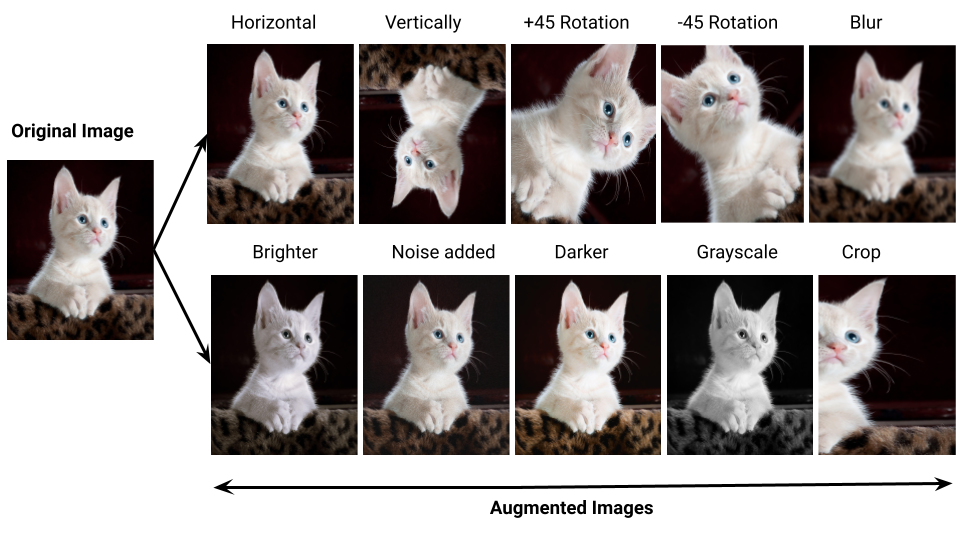
\includegraphics[width=0.6\textwidth]{figures/dataaug.png}
    \end{figure}
\end{frame}

\subsection{Learning Rate Scheduling}
\begin{frame}{}{Learning Rate Scheduling}
    \begin{itemize}
        \item The learning rate is one of the most important hyperparameters to tune for your deep learning model. The learning rate determines how quickly the model learns the optimal weights and how refined the gradient descent process is.
        \item If the learning rate is too high, the model may not converge or converge to a higher loss. If it is too low, the model may take too long to train.

              \only<2>{\item Learning rate scheduling is a technique to adjust the learning rate during training. For example, you can start with a high learning rate and then decrease it over time.}
    \end{itemize}
    \begin{center}
        \begin{tikzpicture}
            \begin{axis}[
                    width=15cm, height=5cm,
                    xlabel={Epochs},
                    ylabel={Loss},
                    ymin=0, ymax=2,
                    xmin=0, xmax=50,
                    legend style={at={(0.97,0.97)},anchor=north east},
                    grid=major,
                    grid style={dashed, gray!30},
                ]

                % Slow reducing loss (low learning rate, lower final loss)
                \addplot [
                    thick,
                    smooth,
                    primary,
                ] coordinates {
                        (0, 1.8)
                        (5, 1.4)
                        (10, 1.0)
                        (15, 0.6)
                        (20, 0.35)
                        (25, 0.25)
                        (30, 0.2)
                        (35, 0.15)
                        (40, 0.1)
                        (45, 0.08)
                        (50, 0.08)
                    };
                \addlegendentry{Low learning rate}

                % Fast reducing loss (high learning rate, higher final loss)
                \addplot [
                    thick,
                    smooth,
                    secondary,
                    dashed,
                ] coordinates {
                        (0, 1.8)
                        (5, 0.9)
                        (10, 0.5)
                        (15, 0.4)
                        (20, 0.35)
                        (25, 0.34)
                        (30, 0.34)
                        (35, 0.34)
                        (40, 0.34)
                        (45, 0.34)
                        (50, 0.34)
                    };
                \addlegendentry{High learning rate}
                \only<2>{
                    \addplot [
                        thick,
                        smooth,
                        tertiary,
                    ] coordinates {
                            (0, 1.8)
                            (5, 0.9)
                            (10, 0.5)
                            (15, 0.4)
                            (20, 0.35)
                            (25, 0.34)
                            (30, 0.34)
                            (32, 0.34)
                            (35, 0.12)
                            (40, 0.1)
                            (45, 0.08)
                            (50, 0.08)
                        };
                    \addlegendentry{Learning rate scheduled} }
            \end{axis}
        \end{tikzpicture}
    \end{center}
\end{frame}

\subsection{Early Stopping}
\begin{frame}{}{Early Stopping}
    \begin{itemize}
        \item Early stopping is a technique to prevent overfitting by stopping the training process when the model's performance on the validation set starts to degrade.
        \item The idea is to monitor the validation loss during training and stop training when the validation loss stops decreasing.
    \end{itemize}
    \vspace{2cm}
    \begin{center}
        \begin{tikzpicture}
            \begin{axis}[
                    width=15cm, height=5cm,
                    xlabel={Epochs},
                    ylabel={Loss},
                    ymin=0, ymax=2,
                    xmin=0, xmax=50,
                    legend style={at={(0.97,0.97)},anchor=north east},
                    grid=major,
                    grid style={dashed, gray!30},
                ]

                % Training loss curve
                \addplot [
                    thick,
                    smooth,
                    primary,
                ] coordinates {
                        (0, 1.8)
                        (5, 1.3)
                        (10, 1.0)
                        (15, 0.7)
                        (20, 0.5)
                        (25, 0.4)
                        (30, 0.3)
                        (35, 0.25)
                        (40, 0.2)
                        (45, 0.15)
                        (50, 0.1)
                    };
                \addlegendentry{Training Loss}

                % Evaluation loss curve
                \addplot [
                    thick,
                    smooth,
                    secondary,
                    dashed,
                ] coordinates {
                        (0, 1.8)
                        (5, 1.4)
                        (10, 1.0)
                        (15, 0.8)
                        (20, 0.6)
                        (25, 0.5)
                        (30, 0.55)
                        (35, 0.6)
                        (40, 0.7)
                        (45, 0.85)
                        (50, 1.0)
                    };
                \addlegendentry{Evaluation Loss}

                % Early stopping marker
                \node at (axis cs: 25,0.5) [pin=above:{Early Stopping Point}] {};

            \end{axis}
        \end{tikzpicture}
    \end{center}
\end{frame}

\subsection{Gradient Clipping}
\begin{frame}{}{Gradient Clipping}
    \begin{itemize}
        \item Gradient clipping is a technique to prevent exploding gradients during training.
        \item Exploding gradients occur when the gradients of the loss function with respect to the model's parameters are too large.
        \item This can cause the model to diverge and fail to learn.
        \item Gradient clipping involves scaling the gradients if their norm exceeds a certain threshold.
    \end{itemize}
    \begin{center}
        \begin{tikzpicture}
            \begin{axis}[
                    width=15cm, height=5cm,
                    xlabel={Epochs},
                    ylabel={Loss},
                    ymin=0, ymax=3,
                    xmin=0, xmax=50,
                    legend style={at={(0.97,0.97)},anchor=north east},
                    grid=major,
                    grid style={dashed, gray!30},
                ]

                % Loss without gradient clipping (with sudden spikes)
                \addplot [
                    thick,
                    smooth,
                    primary,
                    dashed,
                ] coordinates {
                        (0, 2.5)
                        (5, 1.8)
                        (10, 1.3)
                        (15, 0.9)
                        (20, 0.6)
                        (25, 0.5)
                        (28, 1.7)
                        (35, 1.5)
                        (40, 1.3)
                        (45, 1.2)
                        (50, 1.15)
                    };
                \addlegendentry{Without Gradient Clipping}

                % Loss with gradient clipping
                \addplot [
                    thick,
                    smooth,
                    secondary,
                ] coordinates {
                        (0, 2.5)
                        (5, 1.8)
                        (10, 1.3)
                        (15, 0.9)
                        (20, 0.6)
                        (25, 0.4)
                        (30, 0.35)
                        (35, 0.3)
                        (40, 0.25)
                        (45, 0.2)
                        (50, 0.1)
                    };
                \addlegendentry{With Gradient Clipping}

            \end{axis}
        \end{tikzpicture}
    \end{center}
\end{frame}

\subsection{Optimizer Choice}
\begin{frame}{}{Optimizer Choice}
    \begin{itemize}
        \item The choice of optimizer can have a significant impact on the training process and the final performance of the model.
        \item Common optimizers include Stochastic Gradient Descent (SGD), Adam, RMSprop, and Adagrad.
        \item Each optimizer has its own strengths and weaknesses, and the choice of optimizer may depend on the specific problem and dataset.
    \end{itemize}
\end{frame}

\begin{frame}{}{Recall on SGD}
    \begin{itemize}
        \item Stochastic Gradient Descent (SGD) is a variant of gradient descent that updates the model weights using only a small batch of data at each iteration.
        \item The gradient is computed on a mini-batch of data {$(x_i, y_i)$} of size $m$:
              \[
                  g = \frac{1}{m} \sum_{i=1}^{m} \nabla_w L(f(x_i; w), y_i)
              \]
        \item The weights are then updated using the computed gradient:
              \[
                  w = w - \eta g
              \]
              where $\eta$ is the learning rate.
    \end{itemize}
\end{frame}

\begin{frame}{}{RMSprop}
    \begin{itemize}
        \item RMSprop is an adaptive learning rate optimization algorithm that adjusts the learning rate for each parameter based on the magnitude of the gradients.
        \item It maintains a moving average of the squared gradients:
              \[
                  E[g^2]_t = \beta E[g^2]_{t-1} + (1 - \beta) g_t^2
              \]
        \item The weights are then updated using the computed gradient and the moving average:
              \[
                  w = w - \frac{\eta}{\sqrt{E[g^2]_t + \epsilon}} g_t
              \]
              where $\epsilon$ is a small constant to prevent division by zero.
    \end{itemize}
\end{frame}

\begin{frame}{}{Adam}
    \begin{itemize}
        \item Adam (Adaptive Moment Estimation) is an optimization algorithm that combines the benefits of both RMSprop and momentum.
        \item It maintains a moving average of the gradients and the squared gradients:
              \[
                  m_t = \beta_1 m_{t-1} + (1 - \beta_1) g_t
              \]
              \[
                  v_t = \beta_2 v_{t-1} + (1 - \beta_2) g_t^2
              \]
        \item The weights are then updated using the computed gradient and the moving averages:
              \[
                  w = w - \frac{\eta}{\sqrt{v_t} + \epsilon} m_t
              \]
              where $\epsilon$ is a small constant to prevent division by zero.
    \end{itemize}
\end{frame}

\begin{frame}{}{Adagrad}
    \begin{itemize}
        \item Adagrad is an adaptive learning rate optimization algorithm that adjusts the learning rate for each parameter based on the magnitude of the gradients.
        \item It maintains a sum of the squared gradients:
              \[
                  G_t = G_{t-1} + g_t^2
              \]
        \item The weights are then updated using the computed gradient and the sum of squared gradients:
              \[
                  w = w - \frac{\eta}{\sqrt{G_t + \epsilon}} g_t
              \]
              where $\epsilon$ is a small constant to prevent division by zero.
    \end{itemize}
\end{frame}

\begin{frame}{}{Optimizer Comparison}
    \begin{columns}
        \begin{column}{0.4\textwidth}
            \begin{itemize}
                \item SGD is simple and effective, but may require careful tuning of the learning rate and momentum.
                \item RMSprop is effective for non-stationary objectives and works well in practice.
                \item Adam is widely used and often performs well across a variety of tasks, but may not always converge to the optimal solution.
                \item Adagrad is effective for sparse data, but may lead to a rapid decrease in the learning rate.
            \end{itemize}
        \end{column}
        \begin{column}{0.6\textwidth}
            \begin{figure}
                \animategraphics[autoplay,loop,width=0.4\textwidth]{15}{figures/sgd/sgd_}{0}{99}
            \end{figure}
        \end{column}
    \end{columns}
\end{frame}







\subsection{Weight Initialization}
\begin{frame}{}{Weight Initialization}
    \begin{itemize}
        \item Weight initialization is a technique to set the initial values of the weights in the model.
        \item The initial values of the weights can have a significant impact on the training process and the final performance of the model.
        \item If the weights are initialized too small, the model may not learn effectively. If they are initialized too large, the model may not converge.
        \item Common weight initialization techniques include Xavier/Glorot initialization and He initialization.
    \end{itemize}
\end{frame}
\begin{frame}{}{Weight Initialization}
    \begin{itemize}
        \item Xavier/Glorot initialization: The weights are initialized from a normal distribution with mean 0 and variance $2/(n_{\text{in}} + n_{\text{out}})$, where $n_{\text{in}}$ and $n_{\text{out}}$ are the number of input and output units, respectively. It helps prevent the gradients from vanishing or exploding during training by ensuring that the gradients have a similar scale.
        \item He initialization: The weights are initialized from a normal distribution with mean 0 and variance $2/n_{\text{in}}$, where $n_{\text{in}}$ is the number of input units. It is commonly used for ReLU activation functions.
    \end{itemize}
\end{frame}

\subsection{Regularization}
\begin{frame}{}{Regularization}
    \begin{itemize}
        \item Regularization is a technique to prevent overfitting by adding a penalty term to the loss function that discourages the model from learning complex patterns that may not generalize well.
        \item L1 regularization adds a penalty term to the loss function that is proportional to the absolute value of the weights. It encourages sparsity in the weights.
        \item L2 regularization adds a penalty term to the loss function that is proportional to the square of the weights. It encourages the weights to be small.
    \end{itemize}
\end{frame}

\subsection{GPU Acceleration}
\begin{frame}{}{GPU Acceleration}
    CPUs and GPUs are very different in terms of architecture and performance. CPUs are more suited for general-purpose computing tasks, while GPUs are optimized for parallel processing of simple operations, making them ideal for deep learning tasks.
    \begin{itemize}
        \item GPUs are much faster than CPUs for deep learning tasks because they have many more cores and can perform many more operations in parallel.
        \item Deep learning frameworks like PyTorch and TensorFlow are designed to take advantage of GPUs to accelerate the training process.
        \item Only the forward and backward passes of the model are executed on the GPU. The data loading and preprocessing are still done on the CPU.
    \end{itemize}
\end{frame}

